\pagebreak

\section*{Q5}
\begin{solution}
\hfill\break
Code is given after.
\hfill\break
\hfill\break
\textbf{a)} \quad We choose the time-step according to the CFL condition. For the cosine initial condition we note that,
\begin{align*}
    \Delta t &\leq \frac{1}{\text{max} \left| f_u\right|} \Delta x \\
    \text{since }\quad f_u &= \frac{1 + \cos \pi x}{2}, \ \ -1 \leq x \leq 1 \\
    \implies \quad \text{max} \left| f_u\right| &= 1 \\
    \implies \quad  \Delta t &\leq \Delta x
\end{align*}
with a CFL coefficient of $1$.
\hfill\break
\hfill\break
For the triangular wave initialization, we note that,
\begin{align*}
    \text{max} \left| f_u \right| &= \text{max} \left\{ \left|2x - 2\right|, \left|2x + 2\right| \right\}, \ \ -1 \leq x \leq 1 \\
                                  &= 2 \\
    \implies \quad \Delta t &\leq \frac{1}{2} \Delta x
\end{align*}
Thus in this case the CFL coefficient is defined to be $0.5$.
\hfill\break
\hfill\break
The CFL coefficent is defined as a parameter to our function to solve the burgers equation and these values are reflected in the code.
\hfill\break
\hfill\break
\textbf{b)} First we plot the solution to the burgers equation using our exact solver and after we show sketches of the characteristics to show why this happens.
\begin{figure}[H]
    \centering
    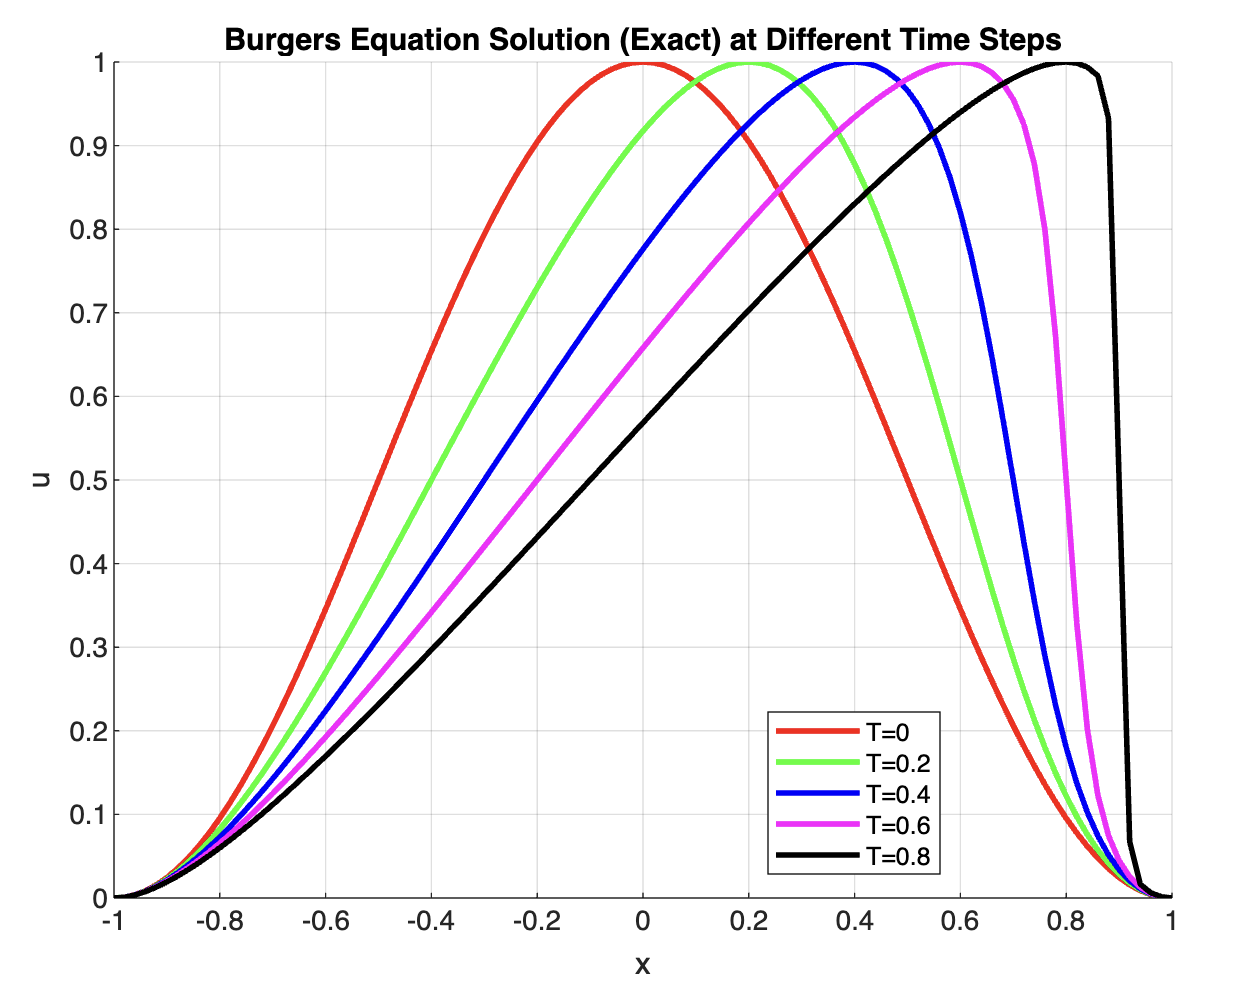
\includegraphics[scale=0.35]{./figures/q5-cos.png}
    \caption{Solving Burgers using exact method and cosine initial conditions.}
\end{figure}
\begin{figure}[H]
    \centering
    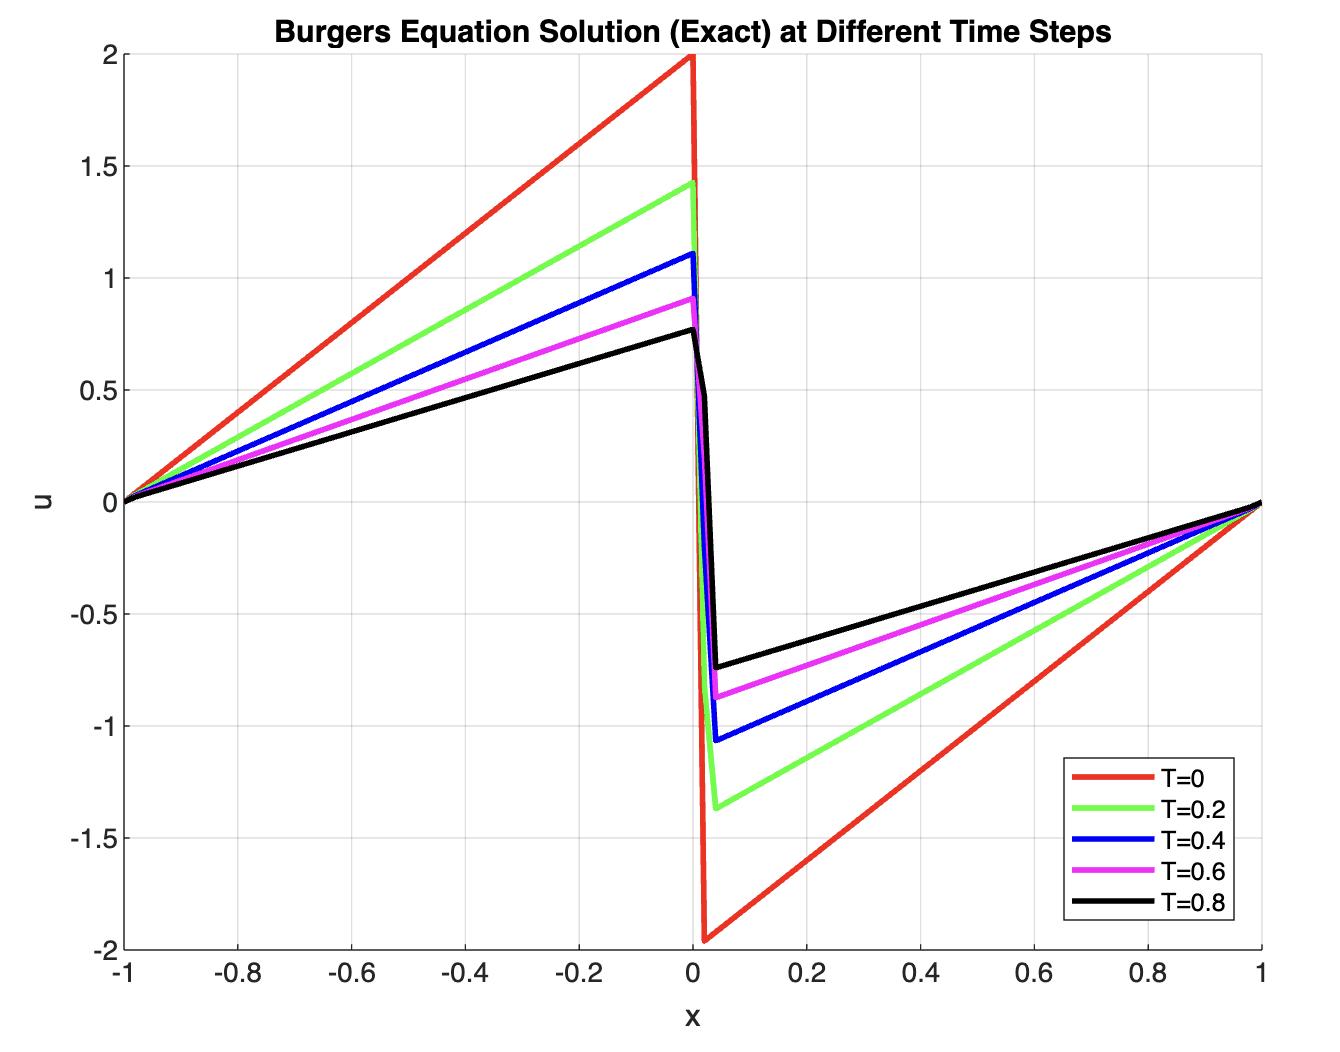
\includegraphics[scale=0.4]{./figures/q5-triangular.png}
    \caption{Solving Burgers using exact method and triangular initial conditions.}
\end{figure}
Now we illustrate the characteristics given the initial conditions for the cosine starting condition and triangular wave starting condition. We see from the overlap and behaviour of the characteristic why non-linear behaviour of the solution exists.
\begin{figure}[H]
    \centering
    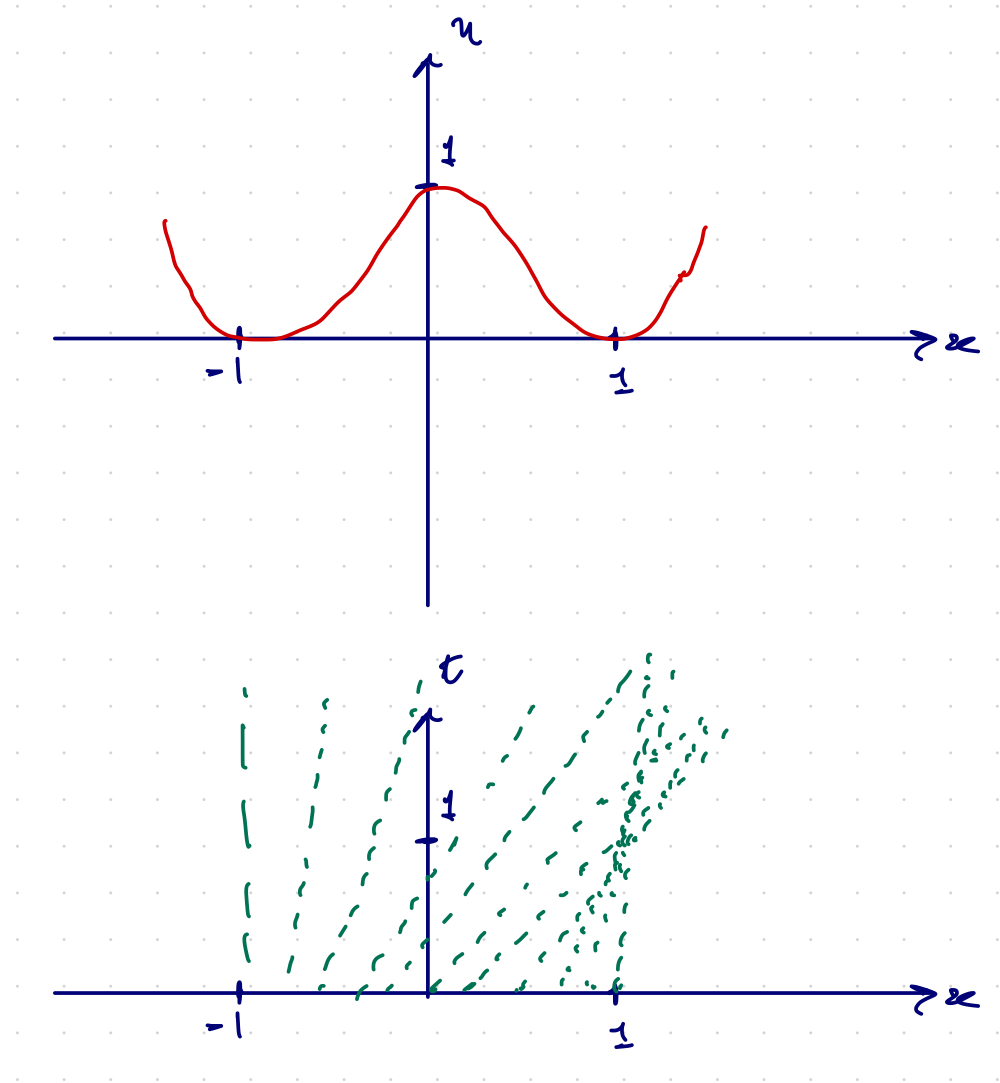
\includegraphics[scale=0.21]{./figures/q5-cos-characteristic.png}
    \caption{First illustrated is $u_{0}(x,0)$ as defined in a) and below is its corresponding characteristic curve graph.}
\end{figure}
\begin{figure}[H]
    \centering
    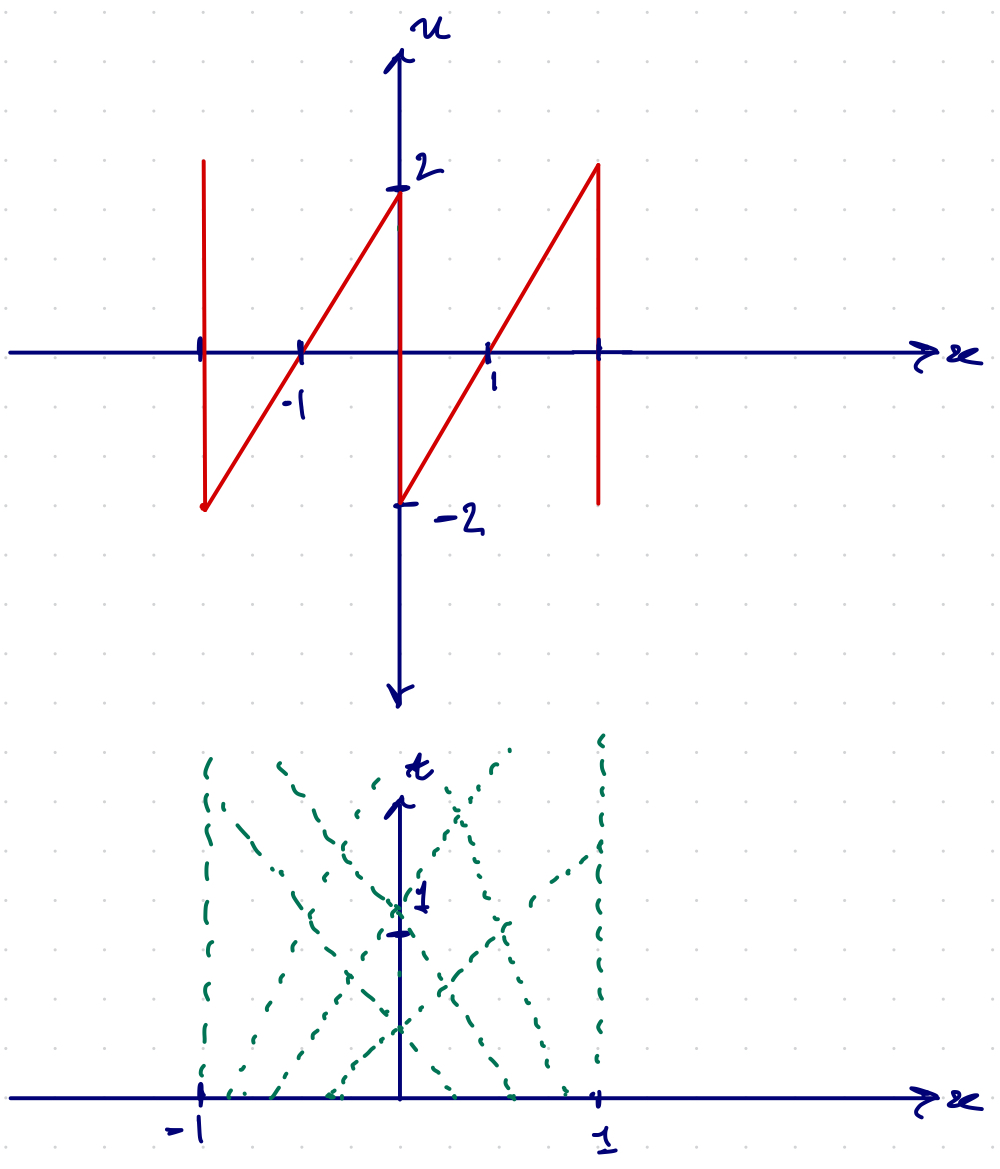
\includegraphics[scale=0.21]{./figures/q5-triangular-char.png}
    \caption{First illustrated is $u_{0}(x,0)$ as defined in b) and below is its corresponding characteristic curve graph.}
\end{figure}
\end{solution}

